\documentclass[14pt]{extarticle}

\usepackage{fontspec}
\usepackage{polyglossia}
\usepackage[a4paper, % Согласно требованиям к ВКР
  lmargin=30mm, rmargin=15mm, tmargin=20mm, bmargin=20mm]{geometry}
\usepackage{multirow}


\setdefaultlanguage{russian}
\setotherlanguage{english}



% Согласно требованиям к ВКР
\defaultfontfeatures{Ligatures=TeX}

\setmainfont{Times New Roman}
\setmonofont{Courier New}
\setsansfont{Arial}

\newfontfamily\cyrillicfont{Times New Roman}
\newfontfamily\cyrillicfontsf{Arial}
\newfontfamily\cyrillicfonttt{Courier New}

\newfontfamily\englishfont{Times New Roman}
\newfontfamily\englishfontsf{Arial}
\newfontfamily\englishfonttt{Courier New}

\linespread{1.5}

\usepackage[backend=biber,
  bibencoding=utf8,
  sorting=none,
  style=gost-numeric,
  language=autobib,
  autolang=other,
  clearlang=true,
  defernumbers=true,
  sortcites=true,
  doi=true,
  isbn=true,
  ]{biblatex}
\bibliography{bibliography}

\usepackage[dvipsnames]{xcolor}
\usepackage[hidelinks,colorlinks=false,citecolor=Black,urlcolor=Black]{hyperref}
\usepackage{caption}
\renewcommand{\UrlFont}{\small\rmfamily\tt}


\renewcommand\thesection{\arabic{section}}

\usepackage{amsfonts}

\usepackage{tikz}
\usepackage{pgfplots}
\usepackage{wrapfig}

\usepackage{graphicx}
\graphicspath{ {./images/} }

\setcounter{secnumdepth}{4}
\setcounter{tocdepth}{4}

% style end

\renewcommand*{\maketitle}{
\begin{titlepage}
  \begin{center}
    \linespread{1}
    \small
    Федеральное государственное автономное образовательное учреждение\break высшего образования\par
    <<Московский физико-технический институт \break (национальный исследовательский университет)>>\par
    Физтех-школа Прикладной Математики и Информатики\par
    Кафедра корпоративных информационных систем\par
  \end{center}
%
  {
    \footnotesize
    {\bf Направление подготовки / специальность}: 01.03.02 Прикладная математика и информатика\newline
    {\bf Направленность (профиль) подготовки}: Прикладная математика и компьютерные науки
  }
%
  {
    \topskip0pt
    \vspace*{\fill}
    \begin{center}
      {\bf\Large Разработка инструмента тестирования
      \break для курса распределенных систем}\par
      (бакалаврская работа)
    \end{center}
    \vspace*{\fill}
  }
%
  \hfill
  \begin{minipage}[t]{8cm}
    {\bf Студент: \newline}
    Поминов Денис Игоревич\newline
    \vspace{-3mm}
    \rule{8cm}{0.15mm}
    \centerline{\scriptsize\it (подпись студента)}\newline
%
    {\bf Научный руководитель: \newline}
    Липовский Роман Германович\newline
    \vspace{-3mm}
    \rule{8cm}{0.15mm}
    \centerline{\scriptsize\it (подпись научного руководителя)}
  \end{minipage}

    \vspace*{\fill}
    \begin{center}
      Москва 2022
    \end{center}
\end{titlepage}
}


\begin{document}
\maketitle

\newpage
\setcounter{page}{2}

\vspace*{\fill}
\begin{abstract}
Тестирование распределенных алгоритмов – важная, но при этом нетривиальная задача из-за  недетерминизма как сети, так и отдельных узлов. Существующие подходы к  тестированию – fault-injection и model checking – по своему несовершенны: либо не покрывают все возможные сценарии исполнения, либо применяются к спецификации алгоритмов, а не тестируют непосредственно реализацию.

Цель данной работы – разработка инструмента для тестирования реализации распределенных алгоритмов, интегрированного в фреймворк курса по распределенным системам. Инструмент должен совмещать сильные стороны существующих подходов: как fault-injection, позволять тестировать непосредственно высокоуровневую реализацию на С++, при этом проверять все возможные состояния исполнения, как model checking.

В работе описана реализация такого инструмента и продемонстрировано его применение на содержательном примере – реализации лианеаризуемого реплицированного атомарного key value хранилища на основе алгоритма ABD.
\end{abstract}
\vspace*{\fill}

\newpage
\tableofcontents
\newpage

\section{Введение}
\label{sec:intro}

На 3 курсе ФПМИ МФТИ проводится курс по распределенным системам. Также этот курс читается на 4 курсе ФКН ВШЭ и 2 курсе ШАД.

При прохождении курса студенты решают практические задачи: написание распределенных сервисов с помощью фреймворка курса whirl \cite{whirl}. Код студентов запускается внутри среды исполнения, которая является детерминированной симуляцией распределенной системы.

Таким образом, основными пользователями фреймворка являются студенты. Далее мы будем отождествлять два этих слова.

Имеется потребность в написании тестирующего инструмента для данного курса распределенных систем. На данный момент тестирование является перебором некоторого количества состояний распределенного сервиса. На некоторых видах задач требуется увеличить покрытие тестирования.

Интеграция фреймворка курса с какими-либо аналогами невозможна, так как фреймворк является самописной разработкой на С++.

\subsection{Постановка задачи}

Инструмент должен решать задачу тестирования распределенной системы, внутри которой исполняется код студента.

Распределенную систему мы представим в виде набора узлов, объединенных в общую сеть. Узлы могут коммуницировать друг с другом только с помощью отправки сообщений.

Сеть мы считаем асинхронной и недетерминированной – она может произвольно задерживать и переупорядочивать отправляемые узлами сообщения. Если система будет корректно работать в асинхронной сети, то и в реальной, частично синхронной сети тоже.

Внутри узла исполняются недетерминированные программы. Также узлы могут отказывать, то есть перезагружаться в произвольные моменты и/или навсегда отключаться.

Мы считаем, что набор узлов системы реализует некоторый распределенный сервис, с которым клиенты взаимодействуют через протокол RPC. 

Клиенты тоже являются узлами сети. 

Они посылают системе запросы и получают ответы, в результате возникает конкурентная история, состоящая из отрезков запросов (рис.~\ref{fig:history_example}). Свойства системы формулируются как утверждения про допустимые истории, которые может порождать система.

\begin{figure}[h]
    \centering
    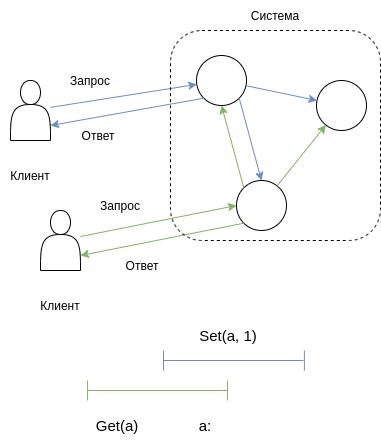
\includegraphics[width=0.5\textwidth]{img/task.png}
    \caption{Пример истории запросов}
    \label{fig:history_example}
\end{figure}

В данной работе нас прежде всего интересует задача репликации, так что распределенный сервис  представляет собой хранилище данных с операциями Set и Get, а свойство, которое мы ожидаем от системы – модель согласованности \cite{consistency}, в первую очередь – линеаризуемость \cite{linearizability}.

Наконец, сформулируем задачу – по реализации узлов системы проверить выполнение заявленных свойств независимо от поведения сети между узлами, часов и т.д.

\subsection{Цель работы}

Цель работы состоит в реализации части библиотеки Roren, отвечающей за перевод и выполнение pipeline-ов поверх YT. Компонент должен позволять запускать произвольные графы обработки данных, выражаемые операциями Map/Reduce.

Получившаяся реализация в сравнении с текущей должна:
\begin{itemize}
    \item Переводить pipeline-ы в графы с меньшим количеством YT операций
    \item Иметь расширяемый на более сложные YT операции алгоритм трансляции
\end{itemize}

\subsection{План работы}

Во второй главе мы рассмотрим дизайн библиотеки Roren: от API pipeline-ов до запуска YT операций.

В третьей главе рассмотрим реализацию компонента, производящего трансляцию. Мы изложим этапы перевода roren графа в граф YT операций, алгоритм трансляции, и детально остановимся на компоненте оптимизатора.

В четвертой главе посмотрим на примеры графов и их трансляций, обсудим тестирование.

В последней главе мы поговорим о результатах работы и обсудим пути развития компонента.


\section{Анализ видов тестирования}
\label{sec:analysis}

Для тестирования недетерминированных распределенных систем и алгоритмов применяются две специальные техники: fault-injection и model checking.

\subsection{Fault-injection}

Fault-injection – техника тестирования недетерминированных конкурентных программ (многопоточных и/или распределенных). Для программы пишется нагрузочный тест, который проверяет наблюдаемые свойства системы (например, модель согласованности), а затем в исполнение этого теста рандомизированно внедряются сбои.

В случае распределенной системы сбоями будут:
\begin{itemize}
    \item Задержка и переупорядочивание сообщений 
    \item Разбиение сети на несколько изолированных друг от друга сегментов, внутри которых сохраняется связность
    \item Отказ узла
    \item Перезагрузка узла, а следовательно, сброс содержимого оперативной памяти
    \item Сдвиг или дрейф локальных часов узла
\end{itemize}

Случайные сбои позволяют увеличить покрытие достижимых в исполнении состояний системы.

Внедрение сбоев может быть реализовано двумя способами: неинвазивный fault-injection и fault-injection в детерминированной симуляции.

Неинвазивность означает, что для тестирования не требуется вносить изменения в код тестируемой системы. Узлы системы запускаются в виртуальном окружении (в отдельных контейнерах), а поведение сети и часов на узлах (сеть и время – основные источники недетерминизма) управляется с помощью системных утилит Linux.

В индустрии стандартом де-факто для неинвазивного fault-injection тестирования распределенных систем является фреймворк Jepsen \cite{jepsen}.

Вариант с fault-injection в детерминированной симуляции состоит в подмене примитивов и абстракций, на которых строится система, для внедрения в них сбоев. У этого подхода есть своя цена – этот тип тестирования должен быть заложен непосредственно в дизайн системы. Примером промышленной системы, которая использует для тестирования fault-injection в симуляции, является база данных FoundationDB \cite{foundation_db}. Также детерминированная симуляция поддерживается в качестве одного из механизмов исполнения в фреймворке курса распределенных систем – whirl-matrix \cite{whirl}.

У техники fault-injection есть очевидное ограничение – рандомизированные сбои не гарантируют, что будут исследованы все возможные состояния, потенциально достижимые в тесте. 

\subsection{Model checking}

Другой подход к тестированию распределенных систем – model checking – состоит в переборе всех достижимых во время исполнения теста состояний системы или алгоритма. 

Все состояния, достижимые в конкретном тесте, можно представить  виде ориентированного графа: 
\begin{itemize}
    \item вершины – конфигурации – описывают мгновенное состояние всей системы, образованное состоянием каждого узла и состоянием сети
    \item дуги в этом графе означают доставку сообщения: при получении сообщения узел меняет свое состояние, возможно отправляя в сеть новые сообщения. 
\end{itemize}

Такой граф назовем графом конфигураций. Каждое конкретное исполнение (обслуживание запросов системой) представляется в графе в виде пути.

Свойства системы имеют разную локализацию в графе конфигураций. Safety свойства – не происходит ничего плохого (например, не нарушается линеаризуемость) – это утверждения про отдельные состояния в этом графе, liveness свойства – когда-нибудь произойдет что-то хорошее (например, при стремлении количества запросов клиентов к бесконечности, количество ответов тоже стремится к бесконечности) – это утверждения про пути в графе.

Задача model checking-а – для теста системы построить граф конфигураций и исследовать выполнение требуемых свойств во всех вершинах или на всех путях этого графа. Компонент, который выполняет такой перебор, назовем model checker.

Когда есть потребность в использовании данной техники, для интересующих критичных частей системы нужно сперва написать спецификацию на формальном языке, которая уже будет проверяться с помощью конкретного инструмента.

В индустрии стандартным инструментом для model checking является формальный язык для написания спецификаций алгоритмов – TLA+ и checker для него – TLC \cite{tla}.

В отличие от fault-injection, эта техника тестирования позволяет гарантированно находить ошибки в алгоритмах. Главный минус подхода – проверяется не реализация системы, а ее спецификация на формальном языке.

\subsection{Выбранный подход}

После анализа был выбран подход, совмещающий сильные стороны обоих техник тестирования. Инструмент – model checker, реализуемый в рамках фреймворка курса распределенных систем, – позволит перебирать все состояния, достижимые в исполнении теста, и обнаруживать нарушения заданных пользователем инвариантов, но при этом будет работать не со спецификацией системы (как TLA+/TLC), а непосредственно с эффективной высокоуровневой реализацией, написанной на языке С++.


\section{Реализация инструмента}
\label{sec:impl}

В этой главе обсуждается устройство инструмента.

\subsection{Дизайн фреймворка курса}

В постановке задачи мы написали, что хотим тестировать реализацию распределенных сервисов. Чтобы такое тестирование было возможным, мы реализуем сервисы в специальном фреймворке (рис.~\ref{fig:runtime}).

\begin{figure}[h]
    \centering
    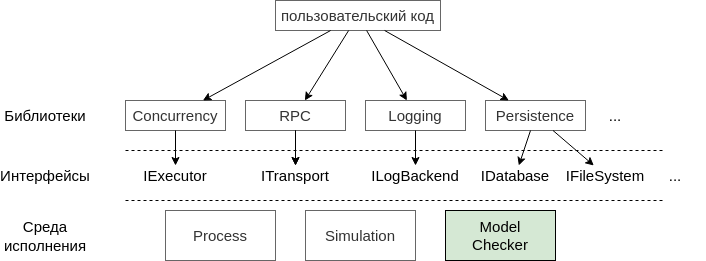
\includegraphics[width=\textwidth]{img/runtime.png}
    \caption{Дизайн фреймворка курса}
    \label{fig:runtime}
\end{figure}

В фреймворке выделяются три уровня:

\begin{enumerate}
    \item Уровень приложения, в котором пользователь описывает свои сервисы с помощью богатого набора высокоуровневых инструментов:
    \begin{itemize}
        \item Отказоустойчивый RPC 
        \item Concurrency (stackful fibers, futures, cancellation)
        \item Инструменты observability: логирование и распределенная трассировка
        \item Persistence (база данных, write-ahead логи, файловая система)
    \end{itemize}
    
    \item Все эти компоненты опираются на небольшой набор базовых абстракций:
    \begin{itemize}
        \item RPC опирается на ITransport – асинхронную шину сообщений для коммуникации между узлами
        \item Concurrency опирается на интерфейс IExecutor – планировщик, исполняющий короткие неблокирующие задачи
        \item Persistence – на интерфейсы IDatabase (локальное KV хранилище) и IFileSystem
        \item и т.п.
    \end{itemize}
    
    \item За реализацию этих интерфейсов отвечает самый низкий уровень – \emph{среда исполнения}.
\end{enumerate}

Среда исполнения, таким образом, отделена от реализации конкретных систем / алгоритмов слоем простых интерфейсов и заключает в себе весь недетерминизм исполнения. Такой дизайн позволяет без изменения пользовательского кода подменять среду исполнения:
\begin{itemize}
    \item процесс-демон с исполнением в многопоточном work-stealing планировщике задач и транспортом сообщений через протокол TCP.
    \item детерминированная симуляция с внедрением сбоев
    \item та часть, разработке которой посвящена работа, model checker.
\end{itemize}

Таким образом, мы получим фреймворк, который сочетает разные подходы к тестированию: и fault-injection, и model checking.

Model checker – это библиотека, которая должна с одной стороны предоставлять узлам системы среду исполнения (сетевой транспорт, планировщик и т.д.), а с другой – представлять собой инструмент с некоторым перебором состояний этого кода.

Реализацию model checker мы разберем с двух сторон: как реализован перебор состояний теста и как реализована среда исполнения для узла распределенной системы, которую пишет пользователь. 

\subsection{Перебор состояний}

Код реализации среды исполнения и код реализации перебора должны быть отделены друг от друга ради того, чтобы иметь возможность писать сколь угодно сложные алгоритмы в checker-е.

\subsubsection{Модель акторов}

Для того, чтобы отделить алгоритм перебора исполнений от среды исполнения для отдельных узлов, будем рассматривать все узлы, на которых подразумевается  исполнение пользовательского кода (как клиентов, так и серверов), в модели акторов \cite{actor}. 

В этой модели все исполняемые сущности (в нашем случае – клиенты и серверы) представляются в виде однопоточных автоматов, которые объединены общей шиной сообщений. Схема взаимодействия внешнего мира с актором такова: актор реагирует на сообщение, адресованное ему, сменой своего состояния и посылкой новых сообщений во внешний мир.

Актор в model checker-е представлен в виде интерфейса IActor с методом HandleMessage (рис.~\ref{fig:actor}): этот метод вызывается model checker-ом. За реализацией этого интерфейса находится узел с пользовательским кодом, RPC и concurrency.

\begin{figure}[h]
    \centering
    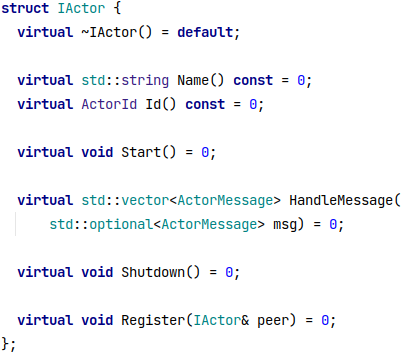
\includegraphics[width=0.75\textwidth]{img/actor.png}
    \caption{Интерфейс актора}
    \label{fig:actor}
\end{figure}

Строго говоря, код пользователя, исполняемый внутри узла, является недетерминированным, и считать узел детерминированным автоматом неверно. Но для model checker-а мы организуем псевдоконкурентное исполнение, оставляя за рамками проверку ошибок многопоточного кода, так как тестирование concurrency является отдельной задачей, для которой применяются те же техники, но в другом масштабе (fault-injection, thread sanitizer).

Стоит представлять себе систему в виде нескольких узлов, которые взаимодействуют через абстракцию физического уровня – сеть. Сеть является глобальным буфером, куда серверы-акторы складывают новые сообщения.

Таким образом, проверка всех достижимых в тесте состояний системы состоит в переборе всех возможных порядков доставки отправляемых узлами-акторами сообщений или, в терминах model checking, в переборе всех возможных ветвей в графе конфигураций.

\subsubsection{Схема перебора}

Model checker может использовать два способа обхода графа конфигураций: поиск в ширину и поиск в глубину. Обход поиском в ширину позволяет находить минимальное по количеству шагов исполнение, нарушающее инвариант \cite{demi}. Минус этого подхода состоит в том, что для него нужно иметь явное представление вершин графа, ведь если сохранять состояние в виде последовательности доставок сообщений, то на очередной итерации BFS приходится снова исполнять доставки в префиксе истории. Обход поиском в глубину позволяет неявно хранить состояние системы: стартуя из начального состояния системы идти по пути, переходя по ребрам за счет доставки сообщений. Мы выбираем обход поиском в глубину, так как из-за ограничения по ресурсам памяти не можем явно хранить состояние сложной распределенной системы.

Деталью перебора является следующее: в начале исполнения очередной ветви мы хотим инициализировать состояние системы, а в конце сбросить текущее состояние. 

В начале перебора ветви выполняется инициализация акторов. В буфер сети на данном этапе приходят все начальные сообщения. Далее происходит перебор, который по описанному алгоритму выбирает очередной индекс сообщения для доставки, извлекает из сети нужное сообщение и доставляет его, тем самым изменяя состояние актора-адресата. После этого буфер, возможно, пополняется новыми сообщениями. На последующих итерациях весь этот процесс повторяется.

\subsubsection{Ограничения}

При тестировании кода нас чаще всего интересует валидация модели согласованности. Такая гарантия является Safety свойством, потому что она представима в виде инварианта через накопление состояния об истории исполнения. Мы сфокусируемся на валидации только такого вида свойств.

Само тестирование будет подразумевать проверку инвариантов кода и не будет работать над проверкой устойчивости кода к перезагрузке узлов, сбоям диска, дрейфу часов и разрывам соединений. Для тестирования подобных сбоев в фреймворке существует режим детерминированной симуляции.

Сбои, состоящие в отказе узла, нет необходимости моделировать отдельно, так как отказ узла – это исполнение, где данный узел не изменяет своё состояние, и ему не доставляются сообщения.

\subsection{Компоненты инструмента}

Теперь обсудим реализацию среды исполнения – рассмотрим каждый логический компонент отдельно.

\subsubsection{Сеть}

Логическая часть model checker-а – сеть – реализует абстракцию связи между серверами. По таким связям проходят сообщения в виде последовательности байт.

Как уже было сказано выше сеть – это глобальный буфер сообщений. Требования к такому буферу состоят в достаточно быстрой доставке произвольного сообщения, то есть извлечению и удалению. 

\subsubsection{Checker}

Далее опишем тот функционал, который ожидался от checker-а и был реализован.

Checker позволяет перебрать все последовательности доставки сообщений в системе, реализуя описанный выше алгоритм перебора.

Во многих тестируемых алгоритмах естественным образом возникают бесконечные ветви в графе конфигураций, что серьезно ограничивает возможность разумного перебора состояний. Для решения этой проблемы была добавлена возможность ограничения глубины пути. В таком сложном случае нужно находить баланс между глубиной пути (а значит временем исполнения) и разумностью количества посещенных состояний.

Нам важна возможность проверки исполнения на детерминизм. Возьмем для проверки некоторую ветвь исполнения.

Основная идея проверки на детерминизм – проверка на то, что состояние системы одинаково после произвольного количества запусков. Состояние системы, как уже было замечено, тяжело представимо в явном виде. Для того, чтобы однозначно понять совпадение состояний, будем поддерживать список активных аллокаций и считать некоторый хэш, комбинируя адреса аллокаций. Делаем три замера: до запуска системы, после первого запуска и после второго. Если дайджесты совпадают, то исполнение гарантируемо детерминировано.

После проверки детерминизма у нас появляется простое неявное представление пути в графе конфигураций – последовательность индексов сообщений для доставки. В таком случае в checker логично добавить возможность исполнения конкретной последовательности доставок с включенным логированием.

\subsubsection{Сервер}

Сервер является реализацией интерфейса актора и объединяет в себе несколько важных компонентов: планировщик, память, транспортный уровень сети, базу данных.

Сервер инициализирует актора через запуск всех запланированных в начальный момент времени задач.

На очередной итерации перебора после доставки сообщения узлу, актор-сервер перенаправляет вызов HandleMessage в реализацию транспортного уровня, которая порождает какое-то количество задач в очереди планировщика. Дальше происходит шаг сервера, состоящий в опустошении очереди планировщика, или на уровне акторов – в переходе в новое состояние в автомате.

\paragraph{Планировщик}\mbox{}

Как уже обсуждалось выше, аналогично задаче построения детерминированной симуляции, нам требуется реализация псевдоконкурентности. Для целей детерминированного исполнения конкурентного кода используется\\ Manual Executor. Такой планировщик представляет собой очередь с задачами, которые планируются в нее из различных мест – fiber-ы, RPC рантайм, коллбэки с кодом пользователя. Далее есть возможность выполнения всех порожденных задач и опустошения очереди, что переводит недетерминированный конкурентный код в state machine.

\paragraph{Память}\mbox{}

Перед тем как рассмотреть реализацию памяти узла, нужно затронуть тему многоразового запуска системы и остановки её в произвольный момент.

Запуск и остановка системы – важная часть checker-а. Перебор строится на возможности множественного перезапуска и остановки системы без утечек памяти.

При завершении исследования ветви в графе конфигураций нам нужно сбросить состояния всех узлов, для этого мы изолируем состояние каждого узла в отдельной куче. Это решение состоит в том, чтобы для узла иметь собственный аллокатор, арену которого в нужный момент можно переиспользовать, затирая все объекты, оставшиеся с прошлых итераций. Более того, различные узлы, для упрощения, могут иметь общий аллокатор, но, в силу разделения их на уровне дизайна, не вторгаться в чужую память.

Итак, память узла – отдельный аллокатор. В реализации используется версия аллокатора с поддержанием списка свободных блоков и простым кэшированием.

В этом месте становится ясно, почему для реализации был выбран язык С++. Помимо необходимости эффективности перебора, нам требуется иметь возможность управлять аллокатором. По этой причине языки со сборкой мусора не подойдут.

\paragraph{Другие компоненты}\mbox{}

Теперь можно поговорить про менее важные компоненты.

Была реализована абстракция транспортного уровня ITransport, благодаря которой возможно легко взаимодействовать узлам по RPC на уровне checker-а. Предоставляются сокеты, возможность подключения к серверу, возможность слушать с некоторым коллбэком на порте. Поддержку disconnect-ов в checker-е можно опустить, так как disconnect одной из сторон – отсутствие доставки некоторого сообщения, что реализуется на уровне алгоритма checker-а.

Поддержание DNS нужно для корректной трансляции адресов транспортного уровня в идентификаторы акторов и наоборот. DNS позволяет нам поддерживать подключение к другим серверам.

Код внутри узла для персистентного хранения данных опирается на интерфейс IDatabase. В model checker-е он реализуется через упорядоченное отображение ключа в значение. Благодаря тому, что мы не моделируем дисковые сбои, отображение – это in-memory map.

Для реализации среды исполнения требуется определить менеджер fiber-ов. Это класс отвечающий за выдачу стеков при создании fiber-а.

\subsubsection{Мир}

Сущности сети и серверов, как акторов, находятся в обобщающем классе, который называется World. Перед запуском перебора исполнений в checker-е в этот класс складываются entry point-ы клиентов и серверов. Мир также содержит в себе бэкенд часть логирования, генератор случайных чисел, поддерживает именованные пулы серверов. Этот класс также хранит предикат для проверки инвариантов. Важной функцией мира является старт и остановка всей системы: серверов, сети, глобальных генераторов (GUID, random).

Генератор GUID является просто монотонным счетчиком.

Сервис генерации случайного числа реализуется стандартным образом через вихрь Мерсенна с возможностью сброса состояния генератора.

Сервис Discovery реализует функцию поиска по названию пула списка адресов серверов, входящих в него, через поддержание такого отображения.

\subsubsection{Логирование поведения}

В фреймворке логирование опирается на интерфейс среды ILogBackend. В инструменте реализовано логирование по уровням для управления детализацией отчета. Минимальный уровень, который будет выводиться в файл, можно задать с помощью переменной окружения. 

Далее происходит захват контекста model checker-а: получение компонента, из которого выполняет логирование, проверка соответствия уровню детализации. На этом этапе происходит формирование структуры Event, в которой собраны номер шага, уровень логирования, краткое описание актора, компонент, в котором вызвано логирование, и само сообщение.

\subsection{Проверка инвариантов}

Задача model checker-а – проверка пользовательских инвариантов во всех достижимых состояниях системы. Пользователь задает инвариант через реализацию интерфейса IPredicate (рис.~\ref{fig:predicate}). IPredicate предоставляет методы сигнала об ошибке Fail, добавления нового непрозрачного состояния Report, проверки корректности предиката IsCorrect и проверки на полноту отчета MakesSense.

\begin{figure}[h]
    \centering
    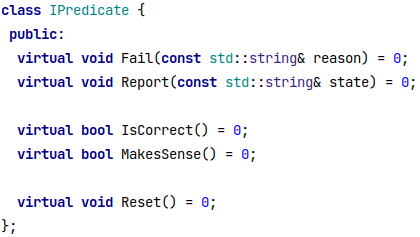
\includegraphics[width=0.75\textwidth]{img/predicate.png}
    \caption{Интерфейс предиката}
    \label{fig:predicate}
\end{figure}

Метод Fail в простейшем случае выполняет роль assert-а. Пользовательский код может просигнализировать таким образом о нарушении инварианта.

Метод Report – добавление нового непрозрачного состояния, которое может интерпретировать только реализация предиката. Такая функция нужна для того, чтобы проверять инварианты не только в каждой вершине, но и на всем пути исполнения в графе конфигураций. К примеру, мы можем с помощью этого механизма выстраивать порядок, в котором операции Set и Get завершались в atomic key value storage. Дальше можно, используя знание о причинности начала операций, написать проверку на линеаризуемость полученной истории.

Проверка корректности IsCorrect нужна по очевидным причинам. Проверка MakesSense на полноту отчета нужна, так как мы хотим иногда ограничивать глубину рассматриваемых исполнений, и это способ снятия метрики количества таких ветвей, чья длина начала превышать лимит, и мы перестали их дальше исполнять.

Мелкой деталью является функция сброса состояния предиката, которую подразумевается использовать при перезапуске системы.

\subsection{Эвристики для ускорения перебора}

Выше была описана наивная реализация model checker-а. На тривиальных примерах была возможность проверить работоспособность инструмента. Но если реализовать какой-либо распределенный алгоритм с использованием RPC сервисов и декомпозицией их на несколько частей, то перебор состояний не завершается за несколько часов. Более того, даже на поиск бага в очевидно неправильном коде затрачивается масса времени.

Далее мы рассмотрим эвристики. Они должны, с одной стороны, не позволять нам упускать содержательные состояния кода. С другой, ускорять перебор и не требовать огромных ресурсов.

\subsubsection{Хэширование состояний}

Напомним, что мы не храним явно состояния системы для перебора. Такая техника подходит под наши ограничения по ресурсам, и она позволяет тратить намного меньше памяти, однако минусом является сложность в поддержании посещенных вершин графа конфигураций. Без этого checker может перебирать экспоненциальное число исполнений, которые имеют совпадающий суффикс, но разный префикс.

В данном случае на помощь приходит хэширование состояний \cite{hash}. Используя стойкую к коллизиям 64-битную хэш-функцию и алгоритм комбинирования хэшей, мы можем быть уверены в небольшом количестве коллизий. Поддержание множества посещенных хэшей дает заметное ускорение.

Для избежания коллизий хэш системы будет являться комбинацией хэшей каждого из узлов и хэша сети. Для комбинации хэшей используется алгоритм hash\_combine из библиотеки boost \cite{boost}. Такой способ составления хэша является некоммутативным и стойким к коллизиям.

Хэш сети – это комбинация хэшей сообщений. Здесь стоит остановится на том, как именно комбинировать хэши сообщений. В исполнениях с разными префиксами, но одинаковыми суффиксами, в сети на момент начала совпадения будут лежать одинаковые сообщения. Однако порядок сообщений будет различным. Поэтому есть два варианта: коммутативный способ комбинирования хэшей сообщений и задание канонического порядка. Как правило, из-за коммутативных хэшей возникает множество коллизий, что критично в нашем случае. Поэтому зададим канонический порядок сортировкой сообщений в сети по хэшу. 

Сортировку производим по запросу хэша от сети. Важно, что сортировка будет проводиться на буфере небольшого объема, так как с ростом числа сообщений количество времени на перебор растет намного быстрее. Поэтому главный параметр выбора алгоритма сортировки – эффективность для маленьких входных данных. Хорошо подходит алгоритм сортировки вставками. Хотя он проигрывает асимптотически другим алгоритмам, на практике на небольшом входе работает быстрее за счет маленькой константы.

Хэш сообщения – хэш полей структуры ActorMessage, которая представляет пакет на сетевом уровне. Хэш пакета вычисляется на стадии его создания, чтобы при запросе хэша сети время затрачивалось только на сортировку и комбинирование пакетов.

Для узла хэшом будет являться хэш памяти и хэш диска. Хэш памяти определяется как хэш аллокатора – комбинация размеров аллокаций для узла. Хэш диска – хэш упорядоченных по ключу пар (ключ, значение) в базе данных, который пересчитывается при каждом выполненном Put. 

\subsubsection{Моментальная доставка ответов}

Для этой эвристики воспользуемся знанием о том, какие сообщения проходят через сеть: запросы и ответы протокола RPC.

С ростом числа сообщений экспоненциально растет число исполнений, т.е. путей в графе конфигураций теста. Мы можем наполовину сократить количество сообщений, если будем доставлять ответы RPC моментально, что сокращает перебор.

\subsubsection{Хэширование памяти узла}

Состояние узла определяется состоянием его диска, его оперативной памяти и регистрами процессоров. Но если учесть, что вся concurrency, написанная в узле является реализацией автомата, а все рассматриваемые алгоритмы (ABD, Raft и т.п.) описываются в виде автоматов, то мы можем не учитывать в хэше точное и сложное состояние исполнения. Достаточно учитывать ключевые переменные, задействованные в алгоритме. А в силу устойчивости алгоритма к рестартам узлов эти переменные уже хранятся на диске узла, так что будем хэшировать только диск.

Например, для алгоритма Raft в спецификации на языке TLA+ можно явно задать то, какие переменные не изменяются при переходах между фазами алгоритма \cite{raft}.


\section{Применение инструмента}
\label{sec:user}

В этой главе мы рассмотрим рекомендации по написанию кода для дальнейшей проверки model checker-ом, опишем тесты, написанные для проверки его корректности, а также примеры использования инструмента на распределенном алгоритме ABD.

\subsection{Написание пользовательского кода}

Перечислим какова последовательность действий для написания теста для model checker-a:

\begin{enumerate}
    \item Написать функцию main узла распределенной системы. В этой функции узел стартует RPC сервер, регистрирует тестируемый RPC сервис и  обслуживает запросы клиентов. Эту функцию будет тестировать model checker.
    \item Написать аналогичную функцию для клиента, которая задает логику теста и те гарантии и инварианты, которые будет проверять model checker через пользовательский предикат.
    \item Также понадобится написать основную функцию, которая будет запускаться с помощью класса Tester. В ней инициализируется объект World, конфигурируются клиенты и серверы системы и, возможно, устанавливается пользовательский предикат.
\end{enumerate}

Функции клиентов и узлов системы. не располагают каким-либо знанием о model checker-е и полагаются только на средства выразительности фреймворка.

В силу того, что практически все алгоритмы репликации используют кворумы, ошибки способны воспроизводиться на небольшом количестве узлов. Нам достаточно использовать 3 сервера и некоторое количество клиентов.

\subsection{Тестирование корректности инструмента}

В первую очередь были написаны синтетические тесты, которые позволили убедиться, что model checker действительно перебирает все достижимые в исполнении теста состояния.

Первый тест (factorial) проверяет, что model checker перебирает все варианты доставки сообщений, одновременно находящихся в сети. Написан клиент, который на старте отправляет в сеть N сообщений с числами от 0 до N-1 и блокируется, ожидая все ответы. Серверная часть – RPC сервис, который имеет единственный метод, принимающий число и сохраняющий его в базу данных, а также логирующий значение. После запуска перебора мы должны получить все перестановки размера N.

Второй тест (ping-pong) – это пинг-понг между серверами: клиент отправляет запрос на один из серверов, этот сервер в свою очередь перенаправляет запрос другому серверу, тот отвечает таким же образом первому. Эта процедура повторяется пока счетчик выполненных запросов не дойдет до установленного лимита. Количество вершин в графе конфигураций вычисляется методом динамического программирования. Совпадение количества исследованных путей и ответа динамики означает, что посещены все состояния.

Следующий тест (livelock) иллюстрирует способность инструмента перебирать все состояния. В качестве сервера выступает сервис атомарной переменной с методами Load, Store, CompareExchange. Клиент реализует поверх такой атомарной переменной мьютекс, гарантирующий взаимное исключение,  но содержащий livelock. В случае графа конфигураций это означает существование бесконечного пути. Model checker находит этот путь и упирается на нем в ограничение глубины.

Последний тест (fetch-add) представляет собой клиента, реализующего операцию FetchAdd поверх сервиса атомарной переменной из прошлого теста через операцию CompareExchange. Одновременно в системе запускается несколько таких клиентов, каждый из которых делает один инкремент. От теста ожидается, что исполнение завершится и в атомарной переменной будет лежать начальное значение плюс количество пользователей. Можно запустить перебор всех состояний такого кода и сравнить суммарное число инкрементов с числом исполнений, умноженным на количество клиентов. В случае корректности model checker-а выполняется равенство.

\subsection{Атомарное key value хранилище (алгоритм ABD)}

Теперь рассмотрим применение model checker-а к нетривиальному примеру – атомарному (линеаризуемому) key-value хранилищу, использующему для репликации алгоритм ABD \cite{abd}.

Алгоритм ABD – решает задачу репликации атомарного регистра с операциями Set и Get, где Set – запись значения по ключу, Get – чтение значения по ключу. Key-value хранилище использует этот алгоритм независимо для каждого ключа.

В данном алгоритме каждая операция отправляет свои запросы на все реплики, но дожидается подтверждения лишь от большинства. Чтения и записи на большинство серверов называются кворумными.

Операция Set – двухфазная: на первой фазе выполняется чтение с кворума реплик и получение максимальной логической временной метки, на второй фазе – кворумная запись значения с выбранной на первой фазе временной меткой.

Операция Get также двухфазная: на первой фазе выполняется кворумное чтение для получения актуального значения, на второй – запись прочитанного значения с максимальной временной меткой. Вторая синхронная фаза не влияет на результат чтения, но необходима для линеаризуемости.

Чтобы model checker был полезным, он должен с одной стороны, находить ошибки в некорректных алгоритмах, а с другой – за разумное время завершать перебор всех состояний в случае корректного алгоритма.

В данном примере model checker должен найти нарушение линеаризуемости в однофазном алгоритме и подтвердить корректность двухфазного.

Клиенты будут делать одинаковые запросы для обоих видов алгоритмов. Один Getter, другой Setter. Работать оба клиента будут с одним ключем “a”. 

Изначально значение по ключу “а” пустое. Setter выполняет операцию Set(“a”, “1”). Getter выполняет последовательно две операции Get(“а”). Исполнение, которое нарушает  свойство линеаризуемости в однофазном алгоритме, устроено так, что операция Set конкурирует с обеими операциями Get.

Для данного примера применимы все эвристики. Отключение хэширования кучи, так как основное состояние – это локальное персистентное хранилище на диске. Моментальная доставка RPC ответов, потому что после отправки запроса реализация алгоритма выполняет блокирующее ожидание ответов.

Минимальный пример строится на трех репликах.

\subsubsection{Однофазный алгоритм}

Рассмотрим нарушение линеаризуемости, которое обнаруживает инструмент. Как обсуждалось выше, нам потребуется два клиента.

На рис.~\ref{fig:one_phase} изображена история доставки сообщений. Операции клиентов изображены сверху и снизу. Три прямые линии посередине – это история (временная ось) каждой из реплик для ключа “а”. Рядом с ключем пишется значение. В случае, если значение пустое, не пишется ничего.

\begin{figure}[h]
    \centering
    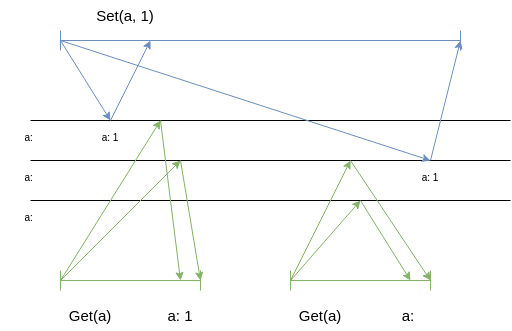
\includegraphics[width=\textwidth]{img/one_phase.png}
    \caption{История для однофазного алгоритма с нарушением линеаризуемости}
    \label{fig:one_phase}
\end{figure}

Для упрощения схемы не будем рисовать первую фазу Set с выбором временной метки, считая что клиент выполняющий Set всего один.

Клиент, дважды выполняющий Get, в результате первой операции прочитал новое значение, а в результате второй – старое. что нарушает линеаризуемость.

На поиск нарушения линеаризуемости model checker с включенными эвристиками затрачивает примерно 1 секунду и 10 MB памяти.

\subsubsection{Двухфазный алгоритм}

Также инструмент тестировался на реализации двухфазной версии алгоритма, которая не нарушает линеаризуемости.

На рис.~\ref{fig:two_phase} изображена история двухфазного алгоритма, которая нарушала свойство для однофазного алгоритма. В данном исполнении первая операция Get не будет завершена пока не произойдет запись нового значения. Это будет гарантировать, что второй Get прочтет новое значение.

\begin{figure}[h]
    \centering
    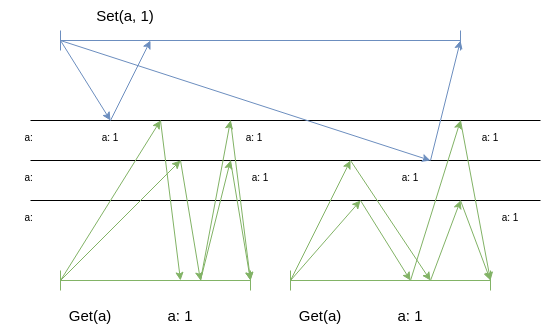
\includegraphics[width=\textwidth]{img/two_phase.png}
    \caption{История для двухфазного алгоритма}
    \label{fig:two_phase}
\end{figure}

В этой версии алгоритма через сеть будет проходить то же количество запросов, что и в однофазной версии, плюс сообщения, порожденные второй фазой операции Get. Полный перебор всех состояний с включенными эвристиками затрачивает примерно 8 минут и 20 MB памяти.

\subsection{Анализ исполнений}

В инструменте есть возможность анализа исполнений с помощью логирования. 

При нахождении нарушения инварианта происходит выход из перебора состояний, включение логирования и ещё одно исполнение последовательности доставок, нарушающих предикат. При этом выводится детализированный лог. Пример на рис.~\ref{fig:log} показывает фрагменты лога с нарушением линеаризуемости в однофазном ABD алгоритме (подчеркнуто красным).

Повторное исполнение последовательности доставок возможно благодаря детерминизму тестируемого кода.

\begin{figure}[h]
    \centering
    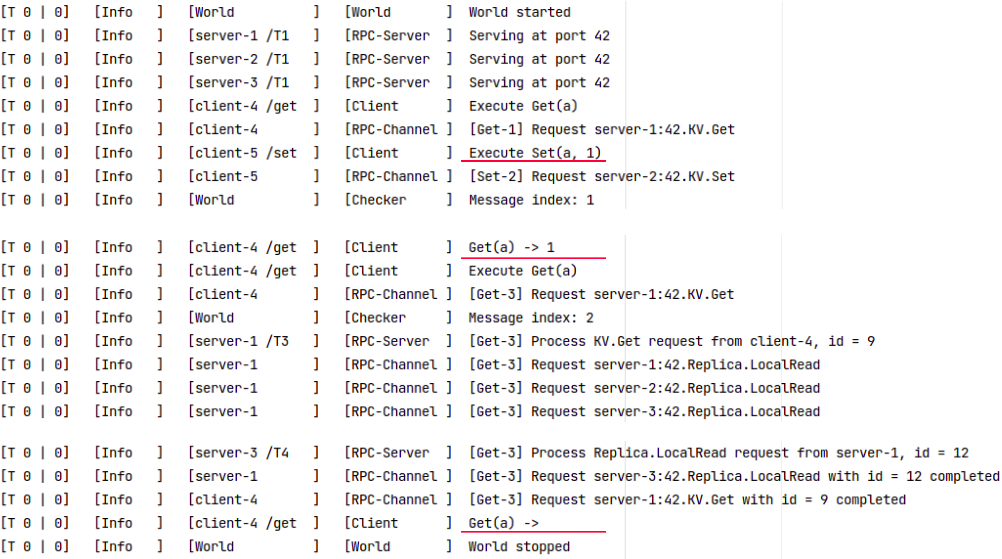
\includegraphics[width=\textwidth]{img/log.png}
    \caption{Лог для однофазного алгоритма с нарушением линеаризуемости}
    \label{fig:log}
\end{figure}


\section{Заключение}
\label{sec:conclusion}

\subsection{Результаты}

Реализован инструмент – model checker, интегрированный в фреймворк курса whirl \cite{checkers}.

Model checker способен проверять инварианты пользовательского кода во время обхода графа конфигураций. При нахождении исполнения нарушающего пользовательский предикат, инструмент выводит детализированный лог.  В написанном model checker-е есть возможность тестирования детерминизма.

Реализация инструмента протестирована на содержательном примере: сервис, реализующий атомарный регистр с помощью алгоритма ABD. Пользовательский код можно писать пользуясь всеми средствами выразительности фреймворка whirl.

Инструмент отрабатывает перебор состояний на нетривиальных примерах за разумное время. При валидации укладывается в лимиты по памяти.


\newpage
\subsection{Планы на будущее}

Задача написания инструмента подобного рода не решается идеально. Основное фундаментальное ограничение – экспоненциальный рост числа состояний с ростом числа сообщений в системе. Существует несколько аспектов, которые можно доработать:

\begin{itemize}
    \item Ускорение алгоритма перебора за счет отсечения симметричных ветвей \cite{dpor}.
    \item Поддержка таймеров. Это возможно сделать через отправку узлом специального сообщения себе.
    \item Визуализация исполнения с нарушением инварианта в виде графа доставки сообщений.
\end{itemize}



\newpage
\printbibliography
\end{document}
